\chapter{Data Acquisition using LabVIEW}

\section{Introduction}
The graphical programming environment LabVIEW \footnote{Laboratory Virtual Instrumentation Engineering Workbench, see http://www.ni.com/labview/} includes a variety of hardware drivers to allow the usage of many different hardware devices. Furthermore LabVIEW is commonly used in data acquisition and instrument control. Platform independent hardware access is an additional benefit of the LabVIEW components. Since it is a graphical environment where the programs and routines are developed and there are lots examples included creating small applications is simple. The modular character of LabVIEW programs allows code reuse without modifications. LabVIEW contains an extra compiler that produces native code for the CPU platform. Therefore it is platform independent and developed programs can easily be deployed on different operating systems like Windows, Mac OS X and Linux. The LabVIEW version used to develop the data acquisition modules was LabVIEW 2011 SP1 (release date 1 March 2012).

\section{Requirements}
The slow control acquisition system collects a variety of different parameters from the experiment, e.g. magnetic field values, vacuum quality, temperature, etc. Additionally it should be possible not only to measure, store and analyze data, furthermore it should be capable of controlling devices. Enable or disable the vacuum pump, open or close valves, etc. To achieve this, there has to be a mechanism that allows the control system to send commands to the devices. Afterwards those commands are processed by the devices.\\

The slow control acquisition handles a slow and permanent submitted data flow. The system should be able to process a data stream with about one data value per second and device. That is way it is called slow control. Beside this data acquisition there is also a fast data acquisition that is not part of this project.\\

The data is stored in a CouchDB database. An access should be possible using so called CouchApps. A big advantage is that those are stored directly in the database and provide a platform independent access since they are mainly written in JavaScript and therefore accessibly through a web browser.\\

The hardware devices should be controllable via short commands that are sent using the database. After inserting such a command, the device should be notified and receive the command instantly. To perform this, it registers to a notification service. Active listening should be avoided.\\

The main part consists of providing a library that handles the interaction and communication with the CouchDB. It provides methods to insert and receive data. Preferably, the library should be platform independent since different operating systems are required to run the experiment properly.\\

\section{Implementation}
\label{section:implementation}
The implementation part of the data acquisition system consists of two different interfaces and the LabVIEW projects. In this chapter the interface 1 from figure \ref{figure:ResultingFramework} as well as the C - library at the device tier are going to be discussed and described in more detail. 

\subsection{LabVIEW VI}
LabVIEW implementations are organized in so-called virtual instruments and represent the programs. In this implementation a VI was developed to show the basic functionality and to fulfill the requirements (insert data and retrieve notifications). A VI consists of two different interfaces. A front panel and a block diagram. The front panel is used for user interaction and to visualize and display information to the user and the block diagram contains the graphical source code. 

\subsubsection{Calling an external function in LabVIEW}
\label{section:callingExtFunction}
To call an external function in LabVIEW a block diagram node called Code Interface Node (CIN) is used \cite{ExtCodeLabView} (see Figure \ref{figure:CIN}a). 
 \begin{figure}[h!]
   \centering
%   \subfiguretopcaptrue
    \subfigure[]
    {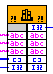
\includegraphics[width=.08\textwidth]{images/CIN.png} \hspace{0.2cm}}
     \subfigure[]
    {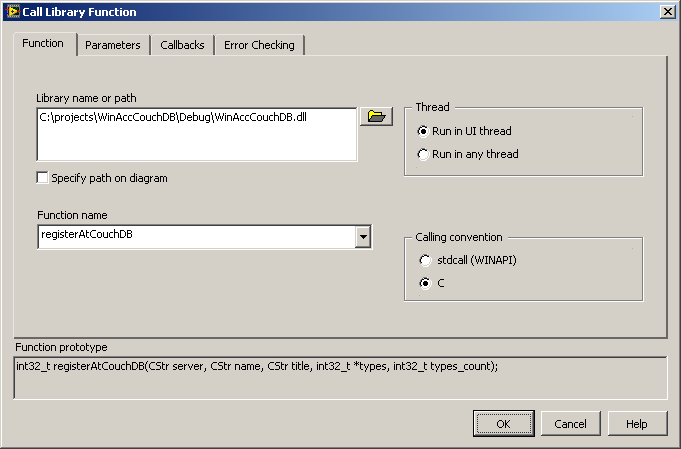
\includegraphics[width=.4\textwidth]{images/CINDetails1.png}\hspace{0.2cm}}
    \subfigure[]
    {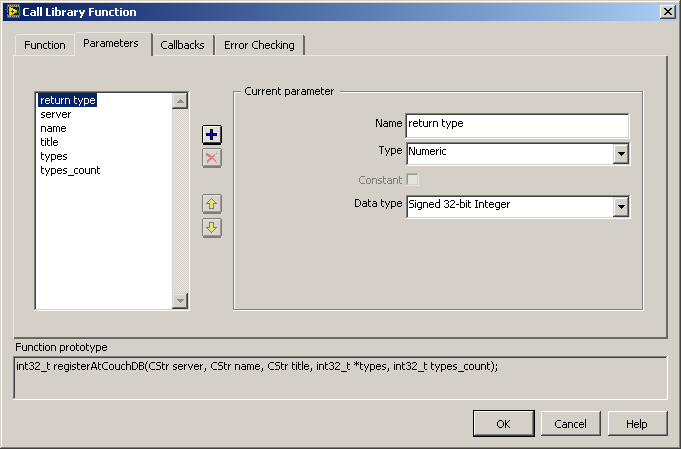
\includegraphics[width=.4\textwidth]{images/CINDetails2.png}}
     \caption{The Code Interface Node and its properties dialog}
     \label{figure:CIN}
  \end{figure}

The CIN can be configured to call a specific function of a C - library. The library can be a Windows library *.dll or a Linux shared object *.so. Within LabVIEW the path to the library is required and additional the header file is necessary to get the parameter lists and functions that are provided by the library. The CIN provides an separate input for every parameter that is expected from the function. Furthermore all inputs need to be connected to some value providing method. This properties can be set in the properties dialog from the CIN. Figure \ref{figure:CIN}a) and b) show the two important tabs of CIN properties. At b) the path to the library and the header file is set. It is also possible to set the calling convention and to the set executing thread. This should be set to the default values. The second tab allows to set the parameters that are necessary to call the function. It is able to set the name, the data type and an option to specify whether it is an array or some numerical value. It is recommended to import a library via the built in function of LabVIEW. The wizard can be found in the menu Tools$\rightarrow$Import$\rightarrow$shared library (.dll) (see Figure \ref{figure:ImportWizard}). The CINs are created automatically and the parameters and return values are set properly\footnote{There is a bug under Windows: if the wizard tries to import a library function that requires some data type from the LabVIEW library "extcode.h". This is the case for the function "InitChangesFeed()". In this case the parameters have to be set manually, whereas the type of the UserEventRef needs to be set to "Adapt to Type".}. To enable a correct import and to call the C - library functions it must be ensured that all libraries that are required can be found. To ensure this, copy all necessary libraries (yajl, libcurl, pillowtalk and in case of Windows pthreadVSE2) in the same folder as the accCouchDB library.

\begin{figure}[h!]
	\centering
		\subfigure[]
      		{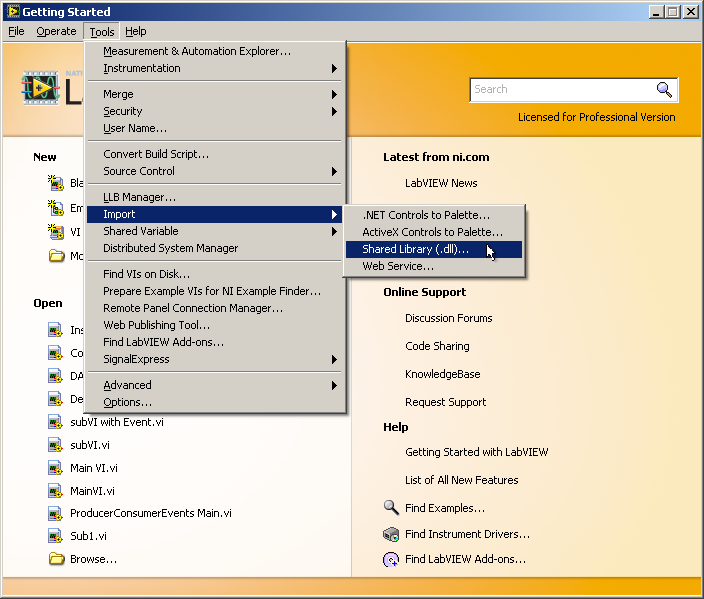
\includegraphics[width=0.4\textwidth]{images/ImportWizard.png}\hspace{1.0cm}}
		\subfigure[]
			{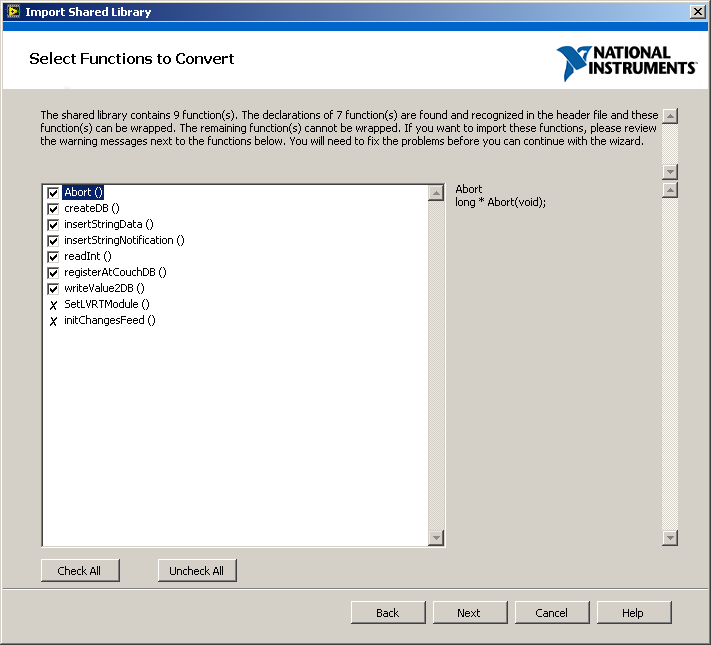
\includegraphics[width=0.4\textwidth]{images/ImportWizard2.png}}
	\caption{Import wizard for shared libraries in LabVIEW}
	\label{figure:ImportWizard}
\end{figure}

\subsubsection{Inserting data and registration of a device}
 
\begin{figure}[h!]
  \centering
      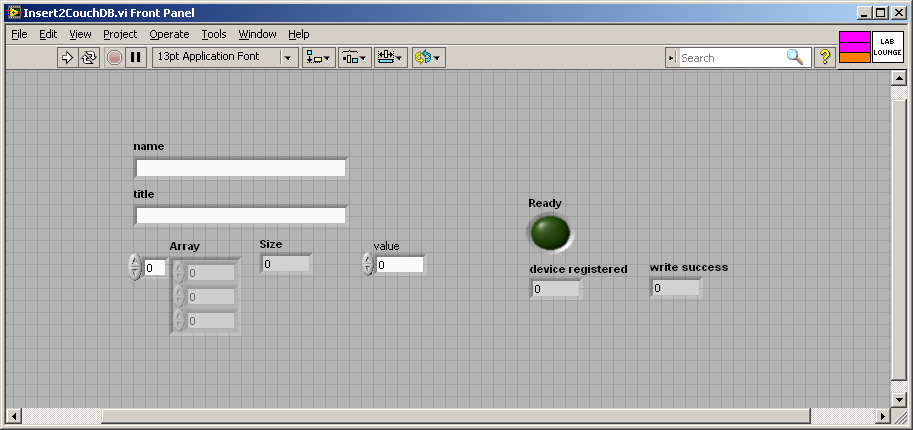
\includegraphics[width=0.9\textwidth]{images/InsertValue2CouchDBfront.png}
  \caption{Front panel of the LabVIEW VI used to register a device and insert a data value.}
  \label{figure:InsertValue2CouchDBfront}
\end{figure}

Figure \ref{figure:InsertValue2CouchDBfront} shows the front panel for a VI that can be used to register a device at the CouchDB and insert a data value. In the front panel the user can specify the name and the title for the device, furthermore an array of numbers can be created to specify the types for one device. After filling the input form the VI can be executed by pressing the "run" button. The program will be executed once and the return values are displayed in the front panel. Figure \ref{figure:InsertValue2CouchDBfrontDone} shows the front panel after the successful execution of the VI. 

\begin{figure}[h!]
  \centering
      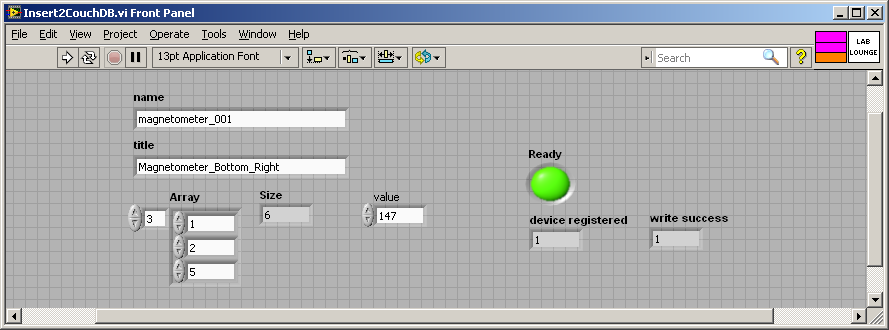
\includegraphics[width=0.9\textwidth]{images/InsertValue2CouchDBfront_done2.png}
  \caption{A VI after a successful device registration and data insertion.}
  \label{figure:InsertValue2CouchDBfrontDone}
\end{figure}

The successful execution can be seen at the two return values. The "device registered" and the "write success" return values are both set to one, which indicates the completion without errors.\\

To see the actual program one have to look at the block diagram. The block diagram consists of the program blocks and represent the functionality of the VI. 

\begin{figure}[h!]
  \centering
      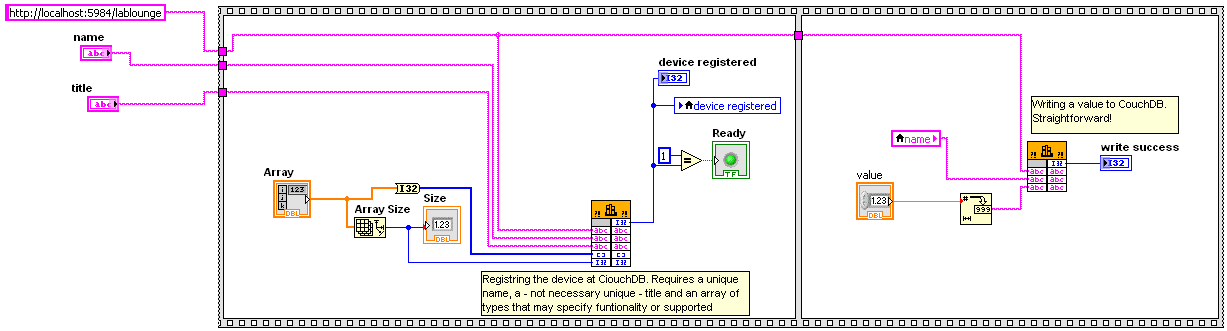
\includegraphics[width=0.9\textwidth]{images/InsertValue2CouchDB.png}
  \caption{The block diagram of the VI.}
  \label{figure:InsertValue2CouchDB}
\end{figure}

The program itself (shown in Figure \ref{figure:InsertValue2CouchDB}) is quite simple. There are only a few methods required to ensure the registration and the insertion of a data value. In principle it consists of two different functions. In the left part of the grey box the device registration is done and afterwards a data value is inserted. The database location is set as a constant. The most important parts are the methods to call an external C function. Those methods require several input parameters and return a value representing the success of the method. The registration in the left part of the grey box needs the location of the database as well as the name and the title of the device. Furthermore an array of numbers can be passed. The result is a number which is displayed in the front panel of the VI (see Figures \ref{figure:InsertValue2CouchDBfront} and \ref{figure:InsertValue2CouchDBfrontDone}). The right part of the grey box handles the insertion of the data value. It requires only the database location and the name of the device and of course the data value, that is going to be stored. The return value is displayed in the "write success" field afterwards. The grey box is a control structure that ensures that the device is registered before it inserts data. The program blocks are executed one after another, beginning with the leftmost block.

\subsubsection{Retrieving notifications from CouchDB}
 
\begin{figure}[h!]
  \centering
      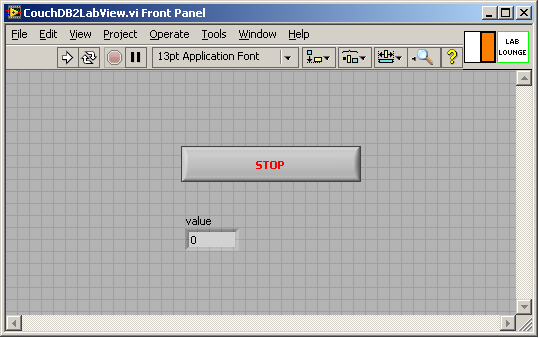
\includegraphics[width=0.4\textwidth]{images/CouchDB2LabVIEWFront.png}
  \caption{Front panel of the LabVIEW VI used to retrieve data values from CouchDB.}
  \label{figure:CouchDB2LabVIEWFront}
\end{figure}

The front panel structure of the VI to retrieve notifications from CouchDB is very simple. It consists of an number indicator to visualize the command that was retrieved and a button to stop the execution and especially the listening thread. 

\begin{figure}[h!]
  \centering
      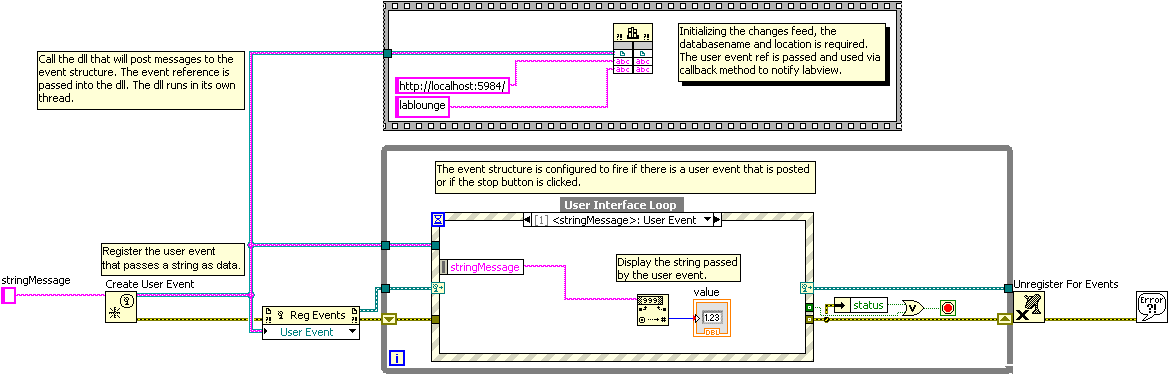
\includegraphics[width=0.9\textwidth]{images/CouchDB2LabVIEW.png}
  \caption{Block diagram of the LabVIEW VI used to retrieve data values from CouchDB.}
  \label{figure:CouchDB2LabVIEW}
\end{figure}

The block diagram (shown in Figure \ref{figure:CouchDB2LabVIEW}) is more sophisticated. It mainly consists of two different execution parts. The upper part is to initialize the thread at the C library. The method requires the location of the database as well as the database name. Furthermore a UserEventReference object is required. This object is created with the function at the very left and used to call the callback function. The UserEventReference is instantiated with an string object as input parameter. As a consequence a string object is expected as parameter in the callback function. The C library is casting every command, that will be sent to LabVIEW, to a string value. The UserEventReference is registered and handled within "User Interface Loop" which handles all events that are generated by the UserEventReference object. Whenever the object fires an event, the content of the stringMessage variable will be read and displayed to the user. The variable could also be read from any other method. Since functions run parallel in LabVIEW changing the stringMessage value causes a VI wide change, so that the change can be seen from everywhere in the VI.\\
\begin{figure}[h!]
  \centering
      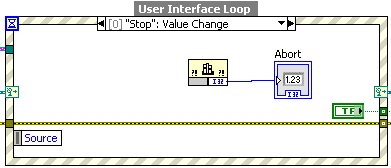
\includegraphics[width=0.5\textwidth]{images/CouchDB2LabVIEW_stop.png}
  \caption{Pressing the stop button terminates the listener thread and the VI.}
  \label{figure:CouchDB2LabVIEWstop}
\end{figure}
The "User Interface Loop" also handles the stop button (see Figure \ref{figure:CouchDB2LabVIEWstop}). If it is pressed by the user the C - library function "Abort" is called an the execution of the thread terminates. This should be done whenever the VI is going to be stopped to ensure that the threads are closed properly and allocated memory is freed. The execution would also stop if there is some error while registering the UserEventReference.

\subsection{C - Library}
The library is accessible on github\footnote{https://github.com/bwaltl}. There are three different repositories available:
 \begin{description}
     \item[accCouchDB] This repository runs on Unix and Windows systems. It provides cross platform compilation using cmake. Additionally it provides all libraries that are necessary to compile under MS Windows. Should be used for further development!
     \item[WinAccCouchDB] This repository is a full Visual Studio 2008 project that produces a version of AccCouchDB library that runs on all Windows systems. 
     \item[UnixAccCouchDB] The Unix version that was created with Eclipse\footnote{http://www.eclipse.org/} and a C/C++ plugin. It produces an shared object library that can be used on Unix systems.
  \end{description}
  
It is recommended to use the cross platform version \textit{accCouchDB}\footnote{https://github.com/bwaltl/accCouchDB} to ensure that changes are made on both, the Unix and MS Windows, versions of the library.

\subsubsection{Building the library}
The library depends on three different other libraries that need to be installed (Unix systems) or otherwise accessible. Anyway they are required to build the AccCouchDB library. 

 \begin{description}
     \item[yajl\footnote{http://lloyd.github.io/yajl/}] A JSON library used to create JSON objects. Necessary to create the communication objects.
     \item[libcurl\footnote{http://curl.haxx.se/libcurl/}] The file transfer protocol library \textit{libcurl} is used to communicate with the CouchDB using URLs. 
     \item[pillowtalk\footnote{https://github.com/mgmarino/pillowtalk/}] ANSI C library that talks to CouchDB using libcurl and yajl.
     \item[pthreadVSE2 (only MS Windows)] On Windows systems an additional threading library is required. Should be available by default. 
  \end{description}
  
Since building these libraries can cause troubles, they are available in the github repositories. In general they should work without great problems, otherwise they have to be created manually following the building instructions of the affected library. \\

After creating a local clone of the AccCouchDB it can be build using the makefile. It is necessary to update the library paths in the \textit{CMakeLists.txt} file that is stored in the \textit{.../AccCouchDB/src/} folder. \\

In MS Windows systems it is sufficient to install the Visual Studio 2008 to ensure that the compiler is available and afterwards start the \textit{Visual Studio 2008 Command Prompt}. To see if the compiler is correctly installed type:\\
\shellcmd{cl}\\
Switch to the folder of the AccCouchDB project and create a build folder:\\
\shellcmd{mkdir build}\\
\shellcmd{cd build}\\
Start the build process by executing the following command:\\
\shellcmd{cmake -G"NMake Makefiles" "..$\backslash$src$\backslash$"}\\
Afterwards the library can be created using the makefile:\\
\shellcmd{nmake}\\
If every step was successfully executed there should be a \textit{AccCouchDB.dll} in the build folder of the project. The corresponding header file \textit{AccCouchDB.h} is in the source folder of the project.\\

In Unix systems it is sufficient to make sure that the gcc compiler is available. To see if the compiler is correctly installed type:\\
\shellcmd{gcc}\\
Switch to the folder of the AccCouchDB project and create a build folder:\\
\shellcmd{mkdir build}\\
\shellcmd{cd build}\\
Start the build process by executing the following command:\\
\shellcmd{cmake "..$\backslash$src$\backslash$"}\\
Afterwards the library can be created using the created makefile:\\
\shellcmd{make}\\
If every step was successfully executed there should be a \textit{AccCouchDB.so} in the build folder of the project. The corresponding header file \textit{AccCouchDB.h} is in the source folder of the project.\\

Beside of all those libraries it is required, that LabVIEW is installed on the operating system. To enable the callback functionality the LabVIEW library \textit{labview.dll} is required. \\
The library file \textit{AccCouchDB.dll} can be used in LabView to communicate with the CouchDB. See chapter \ref{section:callingExtFunction} for more details.

\subsubsection{Functions and implementation}
The C library contains functions, that enable the communication with the CouchDB in a bidirectional way. Basically two things are possible: On the one hand inserting and persisting measured data and on the other hand retrieving notification commands from CouchDB.\\

Inserting data is quite easy and straightforward. This is achieved by calling the function "insertStringData(...)". The function consists mainly of two things, that need to be performed. At the beginning the document has to be created and the proper attributes have to be filled with data. 
\begin{lstlisting}[language=C++]
//create a new document
pt_node_t* root = pt_map_new();

//set the device, that inserts the data
pt_map_set(root, "source", pt_string_new(source));

//retrieve a timestamp
string timestamp = getTimestamp();
pt_map_set(root, "timestamp", pt_string_new(timestamp.c_str()));

//set the data value
pt_map_set(root, "data", pt_string_new(data));
	
//create a unique id 
string id = "data_" + string(source) + getTimestampasID();
pt_map_set(root, "_id", pt_string_new(id.c_str()));
\end{lstlisting}

And the second part of the function is to save the document at CouchDB by calling the \textit{pt\_put(...)} function from pillowtalk.
\begin{lstlisting}[language=C++]
pt_response_t* response = NULL;

//try to insert the document
response = pt_put(keyPath.c_str(), root);
if (response->response_code != 201) {
	log_stringMessage("Data insertion failed", keyPath.c_str());
	log_intMessage("Data insertion failed", response->response_code);
	return OPERATION_FAILED;
}
return OPERATION_SUCCEDED;
\end{lstlisting}

Retrieving notifications from CouchDB can be initialized calling the \textit{initChangesFeed(...)} function. It expects a user reference object, that is stored to call the LabVIEW VI in the callback function.

\begin{lstlisting}[language=C++]
rwer = local_rwer; // store the UserEventRef object

// initialize the changes feed + heartbeat function 
pt_changes_feed_config(cf, pt_changes_feed_continuous, 1);
pt_changes_feed_config(cf, pt_changes_feed_req_heartbeats, 1000);

// register the callback function
pt_changes_feed_config(cf, pt_changes_feed_callback_function, &callback);
pt_changes_feed_run(cf, server, database);
\end{lstlisting}

If an event raises the callback function is called and the most important part there is calling the \textit{PostLVUserEvent(...)} method that is provided by LabVIEW. It requires the UserEventReference object and a string handle object that holds the value that is passed to labview.

\begin{lstlisting}[language=C++]
MgErr result = PostLVUserEvent(*rwer, (void *) &newStringHandle);
\end{lstlisting}

If the execution of a VI stops, the function \textit{abort()} should be called to ensure that the notification threads are halted.\\

Furthermore the library contains more functions to allow different operations. Some of them are useful for development. It is possible to enable or disable logging of the library. Or to create a new database or to insert single data values to a document or read values from a document with a given key. Most of the functions are straightforward and easy to understand. A recommended function that is very useful during the development process is the function \textit{DebugPrintf(...)\footnote{http://zone.ni.com/reference/en-XX/help/371361G-01/lvexcodeconcepts/debugging\_external\_code/}} provided by LabVIEW. It displays string values in a debugging console of LabVIEW and offers a good way to find bugs or other strange behavior in the library functions.

\subsection{A prototypical VI using NI USB-6211}
To combine all the functionality in LabVIEW and to prove the performance of the C library an existing VI was extended to the usage of the DAQ concept of the nEDM. The VI measures a magnetic field and displays the offset and the standard deviation. Those values are logged in a file. The VI was extended to write the value to the CouchDB and to enable or disable the logging function via notification commands sent from CouchDB. \\

\begin{figure}[h!]
  \centering
      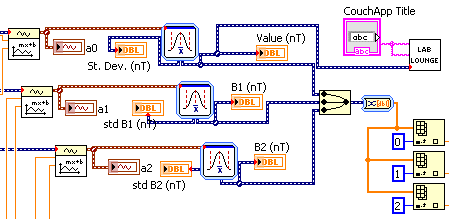
\includegraphics[width=0.4\textwidth]{images/VIExample.png}
  \caption{The insert functionality is encapsulated in a SubVI and only requires a sensor name and the value.}
  \label{figure:ExampleVI}
\end{figure}

Figure \ref{figure:ExampleVI} shows how the functionality can be implemented to an existing VI. The SubVI can be opened by double-clicking on the symbol. The \"CouchApp Title\" is set in the front end of LabVIEW and represents both, the name and the title of the sensor. \\

\begin{figure}[h!]
  \centering
      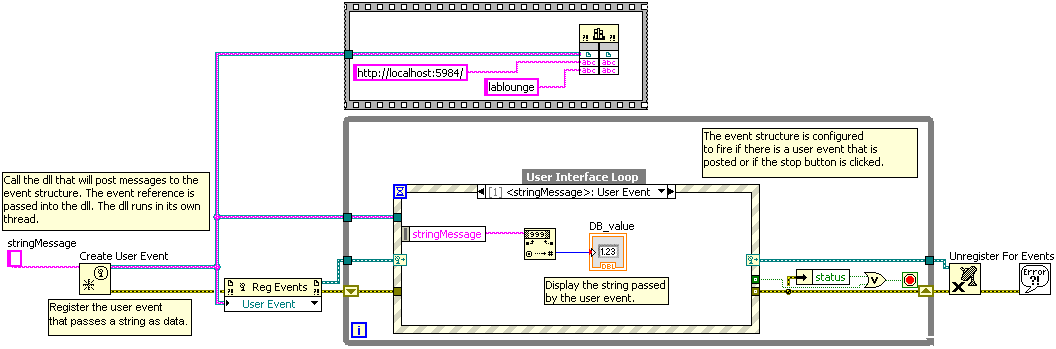
\includegraphics[width=0.9\textwidth]{images/VIExample_notification2.png}
  \caption{Receiving notifications and storing values in a local variable.}
  \label{figure:ExampleVI_receiving}
\end{figure}

Figure \ref{figure:ExampleVI_receiving} represents the functionality of receiving notifications from the CouchDB. After the initialization the event structure is called in case of an event. Afterwards the value that was received is stored in a local variable. \\

\begin{figure}[h!]
  \centering
      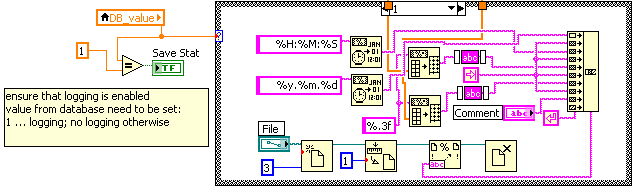
\includegraphics[width=0.5\textwidth]{images/VIExample_notification.png}
  \caption{Logging depends on the value sent from the CouchDB.}
  \label{figure:ExampleVI_receiving}
\end{figure}

Figure \ref{figure:ExampleVI_receiving} shows the VIs logging functionality. If the value of \textit{DB\_value} is set to zero the logging process is no longer executed and therefore no values are stored in a local file.  \\